\documentclass[12pt,a4paper]{amsart}
% ukazi za delo s slovenscino -- izberi kodiranje, ki ti ustreza
\usepackage[slovene]{babel}
\usepackage[T1]{fontenc}
\usepackage[utf8]{inputenc}
\usepackage{amsmath,amssymb,amsfonts,amsthm}
\usepackage{url}
%\usepackage[normalem]{ulem}
\usepackage[dvipsnames,usenames]{color}
\usepackage{graphicx}
\usepackage{tikz}
\usepackage{dsfont}
\usepackage{caption}
\usepackage{subcaption}
\usepackage{bm}
\usepackage{float}

% ne spreminjaj podatkov, ki vplivajo na obliko strani
\textwidth 15cm
\textheight 24cm
\oddsidemargin.5cm
\evensidemargin.5cm
\topmargin-5mm
\addtolength{\footskip}{10pt}
\pagestyle{plain}
\overfullrule=15pt % oznaci predlogo vrstico


% ukazi za matematicna okolja
\theoremstyle{definition} % tekst napisan pokoncno
\newtheorem{definicija}{Definicija}[section]
\newtheorem{primer}[definicija]{Primer}
\newtheorem{opomba}[definicija]{Opomba}

\renewcommand\endprimer{\hfill$\diamondsuit$}


\theoremstyle{plain} % tekst napisan posevno
\newtheorem{lema}[definicija]{Lema}
\newtheorem{izrek}[definicija]{Izrek}
\newtheorem{trditev}[definicija]{Trditev}
\newtheorem{posledica}[definicija]{Posledica}



% ukaz za slovarsko geslo
\newlength{\odstavek}
\setlength{\odstavek}{\parindent}
\newcommand{\geslo}[2]{\noindent\textbf{#1}\hspace*{3mm}\hangindent=\parindent\hangafter=1 #2}


% naslednje ukaze ustrezno popravi
\newcommand{\program}{Finančna matematika} % ime studijskega programa: Matematika/Finan"cna matematika
\newcommand{\imeavtorja}{Anej Rozman} % ime avtorja
\newcommand{\imementorja}{~doc.~dr. Martin Raič} % akademski naziv in ime mentorja
\newcommand{\naslovdela}{Lévijevi procesi z uporabo v financah}
\newcommand{\letnica}{2024} %letnica diplome





\begin{document}

% od tod do povzetka ne spreminjaj nicesar
\thispagestyle{empty}
\noindent{\large
UNIVERZA V LJUBLJANI\\[1mm]
FAKULTETA ZA MATEMATIKO IN FIZIKO\\[5mm]
\program\ -- 1.~stopnja}
\vfill

\begin{center}{\large
\imeavtorja\\[2mm]
{\bf \naslovdela}\\[10mm]
Delo diplomskega seminarja\\[1cm]
Mentor: \imementorja}
\end{center}
\vfill

\noindent{\large
Ljubljana, \letnica}
\pagebreak

\thispagestyle{empty}
\tableofcontents
\pagebreak

\thispagestyle{empty}
\begin{center}
{\bf \naslovdela}\\[3mm]
{\sc Povzetek}
\end{center}
% tekst povzetka v slovenscini

\vfill
\begin{center}
{\bf Lévy processes and their use in finance}\\[3mm] % prevod slovenskega naslova dela
{\sc Abstract}
\end{center}
% tekst povzetka v anglescini
Prevod zgornjega povzetka v angle"s"cino.

\vfill\noindent
{\bf Math. Subj. Class. (2010):} 91G10 60G00 60G01  \\[1mm]
{\bf Klju"cne besede:} Slucajni procesi, Lévijevi procesi   \\[1mm]
{\bf Keywords:} Stochastic processes, Lévy processes
\pagebreak



% tu se zacne besedilo seminarja
\section{Uvod}
    Lévijev proces je slučajni proces imenovan po francoskem matematiku Paulu Lévyju, ki je bil eden od pionirjev na
    področju verjetnosti v 20.\ stoletju. Igral je ključno vlogo pri razumevanju procesov z neodvisnimi, stacionarnimi
    inkrementi (prvotno ime za Lévijeve procese), (dokončaj)

    \begin{figure}[H]
        \centering
        \begin{subfigure}{0.5\textwidth}
            \centering
            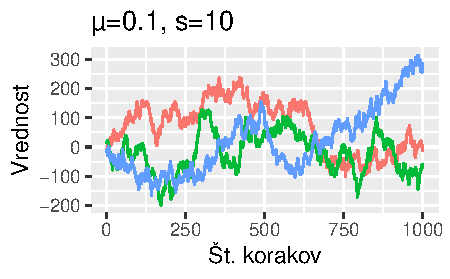
\includegraphics[width=1\linewidth]{C:/Users/38651/OneDrive - Univerza v Ljubljani/Desktop/Diplomski seminar/Levy-Processes/Photos/graphs/BrownGibanje.pdf}
        \end{subfigure}%
        \begin{subfigure}{0.5\textwidth}
            \centering
            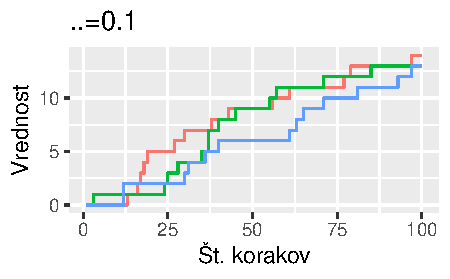
\includegraphics[width=1\linewidth]{C:/Users/38651/OneDrive - Univerza v Ljubljani/Desktop/Diplomski seminar/Levy-Processes/Photos/graphs/PoissGibanje.pdf}
        \end{subfigure}
        \caption{Primera trajektorij Brownovega gibanja in Poissonovega procesa}
        \label{slika1}
    \end{figure}
       
    \noindent
    Zgornji sliki prikazujeta simulacije trajektorij Brownovega gibanja oz. Wienerjevega procesa (levo) in 
    Poissonovega procesa (desno). Oba sta izredno pomembna v svetu financ, Poissonov proces v zavarovalništvu in Brownovo
    gibanje pri vrednotenju finančnih instrumetnov npr.\ opcij. Na prvi pogled ni videti, kot da imata kaj dosti skupnega
    razen dejstva, da sta slučajna procesa. Brownovo gibanje ima zvezne nemonotone trajektorije, medtem ko so trajektorije 
    Poissonovega procesa diskretne in naraščajoče. Kot pa bomo videli, oba zadoščata definiciji Lévijevega procesa. (Ponovno napiši z lepšimi besedami)



\section{Neskončno deljive porazdelitve in Lévy-Hinčinova formula}
    V tem poglavji si bomo ogledali difinicijo neskončno deljivih porazdelitev in njihovo tesno povezavo
    z Lévijevimi procesi. Navedli in dokazali bomo izredno pomemben izrek znan kot Lévy-Hinčinova karakterizacija
    ter pokazali, da velja za Lévijeve procese. (olepšaj in dopolni)
    
    
    \begin{definicija}
        Pravimo, da ima realno številska slučajna spremenljivka $X$ \textit{neskončno deljivo porazdelitev}, če
        za vsak $n \in \mathbb{N}$ obstaja zaporedje neodvisnih enako porazdeljenih slučajnih spremenljivk $(X_i)_{i=1,\dots,n}$, 
        da velja 
        $$
        X \stackrel{d}{=} X_1 + X_2 + \dots X_n,
        $$
        kjer $\stackrel{d}{=}$ pomeni enakost v porazdelitvi.
    \end{definicija}

    \begin{opomba}
        V zgornji definiciji opazimo, da ima $X$ neskončno deljivo porazdelitev, če in samo če velja, da za 
        vsak $n \in \mathbb{N}$, lahko $n$-ti koren karakteristične funkcije $\varphi(X)$ izberemo tako, da 
        je karakteristična funkcija neke slučanjne spremenljivke.
    \end{opomba}

    \begin{lema}
        Linearne kombinacije neodvisnih neskončno deljivih slučajnih spremenljivk so neskončno deljive slučajne spremenljivke.
    \end{lema}


    \begin{proof}
        Za vsak $n \in \mathbb{N}$ lahko zapišemo $X_i \stackrel{d}{=} X_{i_1} + \dots + X_{i_n}$, torej za
        $a_1, \dots, a_n \in \mathbb{R}$ lahko $a_1X_1 + \dots + a_nX_n$ zapišemo kot 
        \begin{align*}
            a_1X_1 + \dots + a_nX_n &\stackrel{d}{=} a_1(X_{1_1} + \dots + X_{1_n}) + \dots + a_n(X_{n_1} + \dots + X_{n_n}) \\
                                    &\stackrel{d}{=} \sum_{i=1}^na_iX_{i_1} + \dots + \sum_{i=1}^na_iX_{i_n}.
        \end{align*}
    \end{proof}

    \begin{definicija}
        Slučajnemu procesu $X = \{X_t \mid t \geq 0\}$ definiranem na verjetnostnemu
        prostoru $(\Omega, \mathcal{F}, \mathds{P})$ pravimo \textit{Lévijev proces}, če zadošča naslednjim pogojem:
        \begin{enumerate}
            \item $\mathds{P}(X_0 = 0)=1$.
            \item Poti $X$ so $\mathds{P}$-skoraj gotovo zvezne z desne (z levimi limitami).
            \item Za $0 \leq s \leq t$ je $X_t - X_s$ enako porazdeljena kot $X_{t-s}$.
            \item Za $0 \leq s \leq t$ je $X_t - X_s$ neodvisna od $\{X_u \mid 0 \leq u \leq s\}$.
        \end{enumerate}
    \end{definicija}

    \begin{definicija}
        \textit{Lévijeva mera} je mera $\Pi$ na $\mathbb{R}\backslash\{0\}$, ki zadošča
        $$
        \int_{\mathbb{R}}(1 \wedge x^2)\Pi(dx) < \infty.
        $$
    \end{definicija}

    \begin{izrek}
        \textbf{(Lévy-Hinčinova formula)} Verjetnostna mera $\mu$ na realni osi je neskončno deljiva s 
        karakterističnim eksponentom $\Phi$,
        $$
        \int_{\mathbb{R}} e^{i\theta x} \mu(dx) = e^{-\Phi(\theta)},\ \text{za} \ \theta \in \mathbb{R},
        $$
        če in samo če obstaja taka trojica $(a, \sigma, \Pi)$, kjer sta $a, \sigma \in \mathbb{R}$ in $\Pi$
        mera na $\mathbb{R}\backslash\{0\}$, ki zadošča $\int_{\mathbb{R}}1 \wedge x^2 \Pi(dx)\leq \infty$, 
        da za vsak $\theta \in \mathbb{R}$ velja
        $$
        \Phi(\theta) = ia\theta + \frac{1}{2}\sigma^2\theta^2 + \int_{\mathbb{R}}(1 - e^{i\theta x} + i\theta x \mathds{1}_{(|x|<1)})\Pi(dx).
        $$
        Še več, trojica $(a, \sigma, \Pi)$ je enolično določena.
    \end{izrek}

    \begin{opomba}
        \begin{enumerate}
            \item V izreku se omejimo na $\mathbb{R}\backslash\{0\}$, da enolično določimo mero $\Pi$. Ekvivalentno bi 
            lahko postavili pogoj $\Pi(\{0\}) = c$ za $c\in \mathbb{R}$ in namesto $\mathbb{R}\backslash\{0\}$ pisali $\mathbb{R}$.
            \item Izbira indikatorja $\mathds{1}_{(|x|<1)}$ v integralu je prav tako pojlubna, saj lahko hitro preverimo, da spremenmba 
            na  $\mathds{1}_{(|x|<c)}$ za $c>0$ spremeni le konstatno $a$.
        \end{enumerate}
    \end{opomba}

    \begin{proof}

    \end{proof}

    \begin{lema}
        Naj bo $X$ neskončno deljiva slučajna spremenljivka in $\varphi_X$ njena karakteristična funkcija. Potem za vsak $z \in \mathbb{C}$.
        velja
        $$
            1 - Re(\varphi_X(2z)) \leq 4(1 - Re(\varphi_X(z)))^2 \qquad \text{in} \qquad 1 - \left|\varphi_X(2z)\right|^2 \leq 4(1 - \left|\varphi_X(z)\right|^2)^2.
        $$
    \end{lema}

    \begin{proof}
        $\int (1 - \cos(2zx))dx = 2 \int (1 - \cos(zx))$
    \end{proof}

    \begin{lema}
        Naj bo $X$ neskončno deljiva slučajna spremenljivka in $\varphi_X$ njena karakteristična funkcija. Potem za vsak $x \in \mathbb{R}$. velja $\varphi_X(x) \neq 0$.
    \end{lema}

    \begin{proof}
        
    \end{proof}

    \begin{izrek}
        Naj bo $X_1, X_2, \dots $ zaporedje neskončno deljivih slučajnih spremenljivk, ki ??? konvergirajo k $X$. Potem je $X$ neskončno
        deljiva slučajna spremenljivka.
    \end{izrek}

% slovar


\section*{Slovar strokovnih izrazov}

%\geslo{}{}
%
%\geslo{}{}
%


% seznam uporabljene literature
\begin{thebibliography}{99}

%\bibitem{}

\end{thebibliography}

\end{document}